%==============================================================================
% presentation.tex
%==============================================================================


%==============================================================================
% Configuration
%==============================================================================

% Internationalisation
\usepackage[utf8]{inputenc}
\usepackage[T1]{fontenc}
% \usepackage[ngerman]{babel}

% Different packages
\usepackage{url}
\usepackage{color,listings,paralist}
\usepackage{enumerate}
\usepackage{tabularx}
\usepackage{alltt}

% Use default Acrobat reader fonts
\usepackage{mathpazo}

% Use CM fonts (increases document size)
\usepackage{ae}

% Use images
\usepackage{graphicx}

% Configure beamer
\usetheme[secheader]{Ikhono}
\usefonttheme[onlylarge]{structurebold}
\setbeamertemplate{navigation symbols}{}

% Variables
\providecommand{\Title}{Parallel Programming}
\providecommand{\Subtitle}{Recitation Session 6}
\providecommand{\Author}{Thomas Weibel <weibelt@ethz.ch>}
\providecommand{\Institute}{Laboratory for Software Technology, \\
  Swiss Federal Institute of Technology Z\"urich}
\providecommand{\Date}{April 15, 2010}

% PDF settings
\hypersetup{
  pdftitle={\Title, \Subtitle},
  pdfauthor={\Author},
  pdfsubject={\Institute},
  pdfkeywords={parallel programming} 
}

% Titlepage
\title{\Title}
\subtitle{\Subtitle}
\author{\Author}
\institute{\Institute}
\date{\Date}

% Listings
\lstdefinestyle{Default}{
  language=Java,
  tabsize=2,
  mathescape=true,
  inputencoding=utf8,
  showstringspaces=false,
  fontadjust=true,
  basicstyle=\ttfamily,
  keywordstyle=\color{blue}\bfseries,
}
\lstset{style=Default}


%==============================================================================
% Document
%==============================================================================

\begin{document}


% Titlepage
\begin{frame}[plain]
  \titlepage
\end{frame}


\section*{Introduction}

\begin{frame}{Executive Summary}
  \begin{itemize}
  \item Formalize understanding of mutual exclusion
  \item Closer look at \lstinline{volatile}
  \item Proof mutual exclusion
  \end{itemize}
\end{frame}


\section{Volatile}

\begin{frame}{Outline}
  \tableofcontents[current]
\end{frame}

\begin{frame}[fragile]{Original Version}
  \begin{lstlisting}
  static int foo;

  void bar () {
     foo = 0;
     while (foo != 255)
       ;
  }
  \end{lstlisting}
\end{frame}

\begin{frame}[fragile]{Optimized Version}
  Compiler will ``optimize'' the previous version:

  \vspace{\stretch{1}}

  \begin{lstlisting}
  static int foo;

  void bar () {
     foo = 0;
     while (true)
       ;
  }
  \end{lstlisting}

  \vspace{\stretch{1}}

  $\Rightarrow$ Infinite loop
\end{frame}

\begin{frame}[fragile]{Volatile}
  With \lstinline!volatile! the loop condition will not be optimized
  away:

  \vspace{\stretch{1}}

  \begin{lstlisting}
  volatile static int foo;

  void bar () {
     foo = 0;
     while (foo != 255)
       ;
  }
  \end{lstlisting}

  \vspace{\stretch{1}}

  The variable is re-read from memory each time it is accessed
\end{frame}

\begin{frame}{Java Language Specification}
  \begin{block}{Volatile}
    A field may be declared volatile, in which case a thread must
    reconcile its working copy of the field with the master copy every
    time it accesses the variable. Moreover, operations on the master
    copies of one or more volatile variables on behalf of a thread are
    performed by the main memory in exactly the order that the thread
    requested.
  \end{block}

  \vspace{\stretch{1}}

  Source: \url{http://java.sun.com/docs/books/jls/second_edition/html/classes.doc.html\#36930}
\end{frame}


\section{Mutual Exclusion Proofs}

\begin{frame}{Outline}
  \tableofcontents[current]
\end{frame}

\begin{frame}[fragile]{Classroom Exercise 1}
  Program for thread \lstinline!A! (\lstinline!myid == 0!)

  \vspace{\stretch{1}}

\begin{lstlisting}
// Thread A
public void run() {
    while (true) {
A1:     non_critical section
A2:     while (!(signal.turn == 0)) {}
A3:     // critical_section
A4:     signal.turn = 1;
    }
}
\end{lstlisting}
\end{frame}

\begin{frame}[fragile]{Classroom Exercise: PingPong}
  Program for thread \lstinline!B! (\lstinline!myid == 1!)

  \vspace{\stretch{1}}

\begin{lstlisting}
// Thread A
public void run() {
    while (true) {
B1:     non_critical section
B2:     while (!(signal.turn == 1)) {}
B3:     // critical_section
B4:     signal.turn = 0;
    }
}
\end{lstlisting}
\end{frame}

\begin{frame}[fragile]{Your Task (Now!)}
  \begin{itemize}
  \item Show that these threads will never be both in their critical
    section at the same time.
  \item You should prove this property in a manner that’s similar to
    the proof given in class.
  \end{itemize}

  \vspace{\stretch{1}}
  
  \begin{center}
    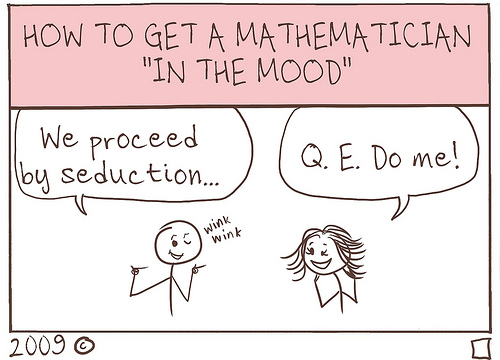
\includegraphics[scale=1.5]{figures/induction} \\
    \tiny{Source: \url{http://brownsharpie.courtneygibbons.org/?p=1146}}
  \end{center}
\end{frame}

\begin{frame}{Some thoughts on how to proceed}
  \begin{itemize}
  \item We introduced already labels for statements and produced two
    distinct versions for thread \lstinline!A! and thread
    \lstinline!B!.
  \item Now you should formulate the invariant.
  \end{itemize}  
\end{frame}

\begin{frame}[fragile]{Invariants}
  \begin{enumerate}
  \item \lstinline!at(A3)! $\rightarrow$ \lstinline!turn == 0!
  \item \lstinline!at(B3)! $\rightarrow$ \lstinline!turn == 1!
  \item \lstinline!not [at(A3) AND at(B3)]!
  \end{enumerate}

  \vspace{\stretch{1}}

  We use the notation ``\lstinline!at(S)!'' to indicate that execution
  is ``at statement (location) \lstinline!S!'' $\Rightarrow$ all
  previous statements have executed while \lstinline!S! has not yet
  started to execute
\end{frame}

\begin{frame}{Proof strategy}
  \begin{itemize}
  \item Proof by induction on the execution sequence.
  \item Base case: does (1) hold at the start of the execution of the
    program (threads at \lstinline!A1! and \lstinline!B1!)?
 \item Induction step: Assume that (1) holds. Will execution of an
   additional step invalidate (1)?
  \end{itemize}
\end{frame}

\begin{frame}{Proof (1)}
  \begin{itemize}
  \item \lstinline!at(A1)!: condition (1) is \lstinline!false!
    $\Rightarrow$ do not care about signal
  \item \lstinline!at(A2)!: condition (1) is \lstinline!false!
    $\Rightarrow$ do not care about signal
  \item \lstinline!at(A3)!: condition (1) is \lstinline!true!
    $\Rightarrow$ \lstinline!turn == 0!, follows from the fact that
    \lstinline!turn!  was \lstinline!0! \lstinline!at(A2)! and the
    transition from \lstinline!A2! $\rightarrow$ \lstinline!A3! did
    not change value of \lstinline!turn!
  \item \lstinline!at(A4)!: condition (1) is \lstinline!false!
    $\Rightarrow$ do not care about \lstinline!turn!
  \end{itemize}

  Now, we consider:

  \begin{itemize}
  \item \lstinline!at(B1)!: no change to \lstinline!turn!
  \item \lstinline!at(B2)!: no change to \lstinline!turn!
  \item \lstinline!at(B3)!: no change to \lstinline!turn!
  \item \lstinline!at(B4)!: changes \lstinline!turn! to \lstinline!0!
  \end{itemize}
  $\Rightarrow$ Invariant (1) is \lstinline!true!
\end{frame}

\begin{frame}{Proof (2)}
  Same way. Please do it if you had trouble with proof of (1).
\end{frame}

\begin{frame}[fragile]{Proof (3): Proof by induction}
  Induction start trivial

  \vspace{\stretch{1}}

  Proof of induction step by contradiction:

  \begin{itemize}
  \item Assume thread \lstinline!A! entered CS (\lstinline!A3!) at time $t1$
  \item Assume thread \lstinline!B! entered CS (\lstinline!B3!) at time $t2$, where $t2 = t1 +
    \delta$
  \end{itemize}

  $\rightarrow$ \alert{Contradiction}: since we are in \lstinline!A3!
  signal \alert{must} be 0 (cannot be 0 and 1 at the same time)

  \vspace{\stretch{1}}

  \begin{itemize}
  \item Assume thread \lstinline!B! entered CS (\lstinline!B3!) at time $t1$
  \item Assume thread \lstinline!A! entered CS (\lstinline!A3!) at time $t2$,
    where $t2 = t1 + \delta$
  \end{itemize}

  $\rightarrow$ \alert{Contradiction}: since we are in \lstinline!B3!
  signal \alert{must} be $1$ (cannot be $0$ and $1$ at the same time)
\end{frame}

\begin{frame}[fragile]{Classroom Exercise 2: Based on 3rd Variation}
\begin{lstlisting}[basicstyle=\fontsize{10}{12}\selectfont\ttfamily]
class Turn {
    // 0 : wants to enter exclusive section
    // 1 : does not want to enter...
    private volatile int flag = 1;

    void request() { 
        flag = 0;
    }

    void free() { 
        flag = 1; 
    }

    int read() { 
        return flag; 
    }
}
\end{lstlisting}
\end{frame}

\begin{frame}[fragile]{Worker}
\begin{lstlisting}[basicstyle=\fontsize{8}{10}\selectfont\ttfamily]
class Worker implements Runnable {
    private int myid;
    private Turn mysignal;
    private Turn othersignal;
    
    Worker(int id, Turn t0, Turn t1) {
        myid = id;
        mysignal = t0;
        othersignal = t1;
    }
    public void run() {
        while (true) {
            mysignal.request();
            while (true) {
                if (othersignal.read() == 1) break;
            }
            // critical section
            mysignal.free();
        }
    }
}
\end{lstlisting}
\end{frame}

\begin{frame}[fragile]{Master}
\begin{lstlisting}
class Master {
    public static void main(String[] args) {
        Turn gate0 = new Turn();
        Turn gate1 = new Turn();
        Thread t1 = 
            new Thread(
                new Worker(0, gate0, gate1)
            );
        Thread t2 = 
            new Thread(
                new Worker(1, gate1, gate0)
            );
        t1.start();
        t2.start();
    }
}
\end{lstlisting}
\end{frame}

\begin{frame}[fragile]{Worker 0}
\begin{lstlisting}
public void run() {
    while (true) {
A1:
A2:     s0.request();
A3:     while (true) {
            if (s1.read() == 1) 
                break;
        }
A4:     // critical section
A5:     s0.free();
    }
}
\end{lstlisting}
\end{frame}

\begin{frame}[fragile]{Worker 1}
\begin{lstlisting}
public void run() {
    while (true) {
B1:
B2:     s1.request();
B3:     while (true) {
            if (s0.read() == 1) 
                break;
        }
B4:     // critical section
B5:     s1.free();
    }
}
\end{lstlisting}
\end{frame}

\begin{frame}[fragile]{Mutual exclusion}
  Show that this solution provides mutual exclusion.
\end{frame}

\begin{frame}{Invariants}
  \begin{enumerate}
  \item \lstinline!s0.flag == 0! equivalent to
    \lstinline!(at(A3) $\text{ }\vee\text{ }$ at(A4) $\text{ }\vee\text{ }$ at(A5))!
  \item \lstinline!s1.flag == 0! equivalent to
    \lstinline!(at(B3) $\text{ }\vee\text{ }$ at(B4) $\text{ }\vee\text{ }$ at(B5))!
  \item \lstinline!not (at(A4) $\text{ }\wedge\text{ }$ at(B4))!
  \end{enumerate}
\end{frame}

\begin{frame}[fragile]{Induction}
  Show with induction that (1), (2), and (3) hold.

  \vspace{\stretch{1}}

  At the start, \lstinline!s0.flag == 1! and \lstinline!at(A1)!
  $\Rightarrow$ {\color{green} OK}

  \vspace{\stretch{1}}

  Induction step: assume (1) is true. Consider all possible moves

  \begin{itemize}
  \item \lstinline!A1 $\rightarrow$ A2!
  \item \lstinline!A2 $\rightarrow$ A3!
  \item \lstinline!A3 $\rightarrow$ A3!
  \item \lstinline!A3 $\rightarrow$ A4!
  \item \lstinline!A4 $\rightarrow$ A5!  
  \item \lstinline!A5 $\rightarrow$ A1!
  \end{itemize}

  \vspace{\stretch{1}}

  Let's look at them one by one:
\end{frame}

\begin{frame}[fragile]{Induction Step}
  \begin{itemize}
  \item \lstinline!A1 $\rightarrow$ A2!: no effect on (1)
    $\Rightarrow$ {\color{green} OK}
  \item \lstinline!A2 $\rightarrow$ A3!: (1) holds
    (\lstinline!s0.flag == 0! and \lstinline!at(A3)!) $\Rightarrow$
    {\color{green} OK}
  \item \lstinline!A3 $\rightarrow$ A3!: (1) holds, no change to
    \lstinline!s0.flag!, \lstinline!at(A3)! $\Rightarrow$
    {\color{green} OK}
  \item \lstinline!A3 $\rightarrow$ A4!: (1) holds, no change to
    \lstinline!s0.flag!, \lstinline!at(A4)! $\Rightarrow$
    {\color{green} OK}
  \item \lstinline!A4 $\rightarrow$ A5!: (1) holds, no change to
    \lstinline!s0.flag!, \lstinline!at(A5)! $\Rightarrow$
    {\color{green} OK}
  \item \lstinline!A5 $\rightarrow$ A1!: (1) holds,
    \lstinline!s0.flag == 1! and \lstinline!at(A1)! $\Rightarrow$
    {\color{green} OK}
  \end{itemize}

  \vspace{\stretch{1}}

  Note that the ``$\Rightarrow$ {\color{green} OK}'' is based on the
  observation that no action by Thread Worker 1 will have any effect
  on \lstinline!s0.flag!

  \vspace{\stretch{1}}

  $\Rightarrow$ So (1) holds.
\end{frame}



\begin{frame}{Your turn}
  Show that (2) holds as well.
\end{frame}

\begin{frame}[fragile]{Proving (3)}
  Proof by induction

  \vspace{\stretch{1}}

  At the start, \lstinline!at(A1)! and \lstinline!at(B1)!, so (3)
  holds.

  \vspace{\stretch{1}}

  Induction step: assume (3) holds and consider possible transitions.

  \vspace{\stretch{1}}

  Assume \lstinline!at(A4)! and consider
  \lstinline!B3 $\rightarrow$ B4! \\
  (while \lstinline!Worker0! remains at \lstinline!A4!!)

  $\Rightarrow$ no other transition is relevant or possible

  \vspace{\stretch{1}}

  But since \lstinline!s0.flag==0! (because of (1)), a transition
  \lstinline!B3 $\rightarrow$ B4! is not possible, so (3) remains
  true.
\end{frame}

\begin{frame}{Proving (3)}
  Same argument applies if we start with the assumption
  \lstinline!at(B4)!.

  \vspace{\stretch{1}}

  So no transition will violate (3).

  \vspace{\stretch{1}}

  Of course this proof sketch depends on the fact that

  \begin{itemize}
  \item no action of \lstinline!Worker0! will modify any of the states
    of \lstinline!Worker1!, and
  \item no action of \lstinline!Worker1! will modify any of the states
    of \\
    \lstinline!Worker0!
  \end{itemize}
\end{frame}


\section*{Outro}

\begin{frame}{Summary}
  \begin{itemize}
  \item Mutual exclusion
  \item Volatile in Java
  \item Proofs for mutual exclusion
    \begin{itemize}
    \item Try to solve assignment 6 -- there will be at least one
      proof at the exam
    \end{itemize}
  \end{itemize}

  \vspace{\stretch{1}}
  
  \begin{center}
    
\includegraphics[scale=0.18]{figures/dilbert}
  \end{center}
\end{frame}

\end{document}
